\documentclass[7x9]{times}

% use mit book class




\title{Penetration Testing and Ethical Hacking}
\author{Many authors}
%\institude{Nanjing University, China}
\date{\today}
\edition{2019 Edition}



%% For multiple indices:
%\usepackage{multind}
%\makeindex{topics}
%\makeindex{authors}

\def\taupav{\tau_{\mathrm{Pav}}}

\newbox\oiintbox
\setbox\oiintbox=\hbox{$\lower2pt\hbox{\huge$\displaystyle\circ$}
	\hskip-13pt\displaystyle\int\hskip-7pt\int_{S}\ $}
\def\oiint{\copy\oiintbox}

\def\boldnabla{\hbox{\boldmath$\displaystyle\nabla$}}

\nocropmarks

\usepackage{multind}
\makeindex{topics}
\makeindex{authors}

\usepackage{listings}
\lstloadlanguages{bash,Python}

\usepackage[caption=false,font=footnotesize]{subfig}

\begin{document}

%[frontmatter] turns off chapter numbering and uses roman numerals for
%page numbers; [mainmatter] turns on chapter numbering, resets page
%numbering and uses arabic numerals for page numbers; [appendix]
%resets chapter numbering, uses letters for chapter numbers and
%doesn't fiddle with page numbering; [backmatter] turns off chapter
%numbering and doesn't fiddle with page numbering.

\titlepage

\begin{copyrightpage}

  \copyright\ 2019 Center for Cybersecurity and Cybersecurity Malaysia
	
	All rights reserved. No part of this book may be reproduced in
        any form or by any electronic or mechanical means (including
        photocopying, recording, or information storage and retrieval)
        without permission in writing from the publisher.
	
	
	This book was set in Minion Pro and Myriad Pro by the author.
	
	Printed and bound in the United States of America.
	
	MIT License. This work is licensed under a Creative Commons Attribution 
	4.0 International License.
	
	Penetration Testing and Ethical Hacking/ .\\
	\hspace*{6pt} p. cm.
	
	Includes bibliographical references and index.\\ ISBN ????
        \vfill
	
	10\ 9\ 8\ 7\ 6\ 5\ 4\ 3\ 2\ 1\
	
\end{copyrightpage}

\tableofcontents
\listoffigures
\listoftables

\begin{contributors}[twocolumn]
	
	\contrib 
	Mohd Zamri Murah\\
	Center for Cybersecurity\\
	Universiti Kebangsaan Malaysia
	
	\contrib 
	Professor Andrei Linde\\
	Department of Physics\\
	Stanford University\\
	Stanford, CA, USA
\end{contributors}


\begin{preface}

ALhamduiLlah. This book is based on lecture notes for
\textit{TX6244:Ethical Hacking and Penetration Testing}, a course
offered by Center for Cybersecurity(UKM) since 2014. This course is
jointly developed by Center for Cybersecurity(UKM) and Cybersecurity
Malaysia(CSM).

We hope this book will provide a good overview for students into the
field of penetration testing and ethical hacking. We also hope these
materials will encourage students to further explore this exciting
field.

We try hard to be current up to 2019. However, this is a tall order
with the amount of information available on the Internet. Al always,
please inform of any errors or omissions to \url{zamri@ukm.edu.my}.

The book source code is available on
\url{github.com/mohdzamrimurah/bukusiber}, and we welcome
collaboration from all users.



\end{preface}

\chapter{Introduction to Ethical Hacking}

\paragraph{Cyber attacks} have increasing common in the past years. Many of these attack
targeted business entities, government websites, financial institutions, 
social network sites, power utilities, education sites and other sites. These attack could cause financial lost, data breach, lost of consumer confidence, dan other risks. Because
of the increase frequency and the severity of the cyber attacks, many organization begin to
take proactive measure to assess their own network security status. One of these proactive
step is penetration testing.

Penetration testing, or ethical hacking, is a process to assess the security level of an organization. It consists of structure steps on how to hack or to break into the organization
network, websites or it infrastructure by simulating external cyber attacks on the 
organization. The main purpose of a penetration testing is to discover securities issues
that could be exploited by cyber hackers and to offer counter measures to these risks.

\section{Cyber attacks}

\paragraph{18/1/2019} A collection containing more than 87 gigabytes of personal information was leaked online. The data dump had 772,904,991 email addresses, and 21,222,975 passwords. Data breaches continue to happen as companies collect data on millions of people and fail to protect them properly. Marriott loss personal information belonging to 383 million guests, Yahoo data belonging to 3 billion accounts were stolen. About 147.7 million Social Security numbers taken in the Equifax data breach.

% https://www.zdnet.com/article/
% singapore-suffers-most-serious-data-breach-affecting-1-5m-
% healthcare-patients-including-prime/
\paragraph{In Singapore}, 1.5 million patients of SingHealth had been accessed and copied. The stolen data included patients' name, national identification number, address, gender, race, and date of birth. Also, outpatient medical data of some 160,000 patients were compromised. Hackers had gained control through breaching a frontend workstation, from which they then were able to obtain privileged account credentials to gain access to SingHealth's database. Cybersecurity vendors have warned that the compromised data may find its way on the Dark Web.


\section{Definitions}




\chapter{Tools and Software}


\paragraph{Tools and Software} This chapter contain
information about basic essential tools and software for penetration
testing. Familiarity of these tools would make it easier to conduct
penetration testing.


\section{Linux}

Linux\cite{sobell2015practical,barrett2016linux} is an operating
system for computer, much like Window 10 or Mac OSX. It is based on
Unix. Linux was first developed in 1991 by Linus Torvalds, a Finnish
graduate student. Currently it is being develops and maintains by a
group of software developers head by Linus Torvalds. It is widely uses
in large technology companies like Google, Facebook, and Amazon. Linux
is widely use as enterprise servers for enterprises daily
operation. It is estimated that 70\% of web servers use Linux, with
30\% using Window-based servers.

Linux is open source and free for everybody to use and to modify. The
open source creative license make it possible for any person or
organization to modify Linux to fit their needs. For instance, Chinese
government produce their own modified version of Linux for the Chinese
market(\url{http://www.kylinos.com.cn/}). Similarly, many organization
such as NSA, Google(\url{gLinux}), Amazon have customized Linux for
their need. Figure~\ref{fig:ubuntu} shows a Linux Ubuntu desktop.

There are many Linux distributions such as Ubuntu, SuSE, Debian and
Red Hat. Red Hat(Linux) is widely use as enterprise servers, Ubuntu is
widely by customer desktop and Debian is normally uses by software
developers. A Linux distribution is a Linux operating system with
other useful software such such text editor, pdf viewer, browser,
music player and image processing. A Linux distribution is similar to
a PC with Window 10, Microsoft Office software and other familiar
software applications.

\index{topics}{Linux}
\index{topics}{Kali Linux}

%\begin{center}
%	\begin{figure}[]
%		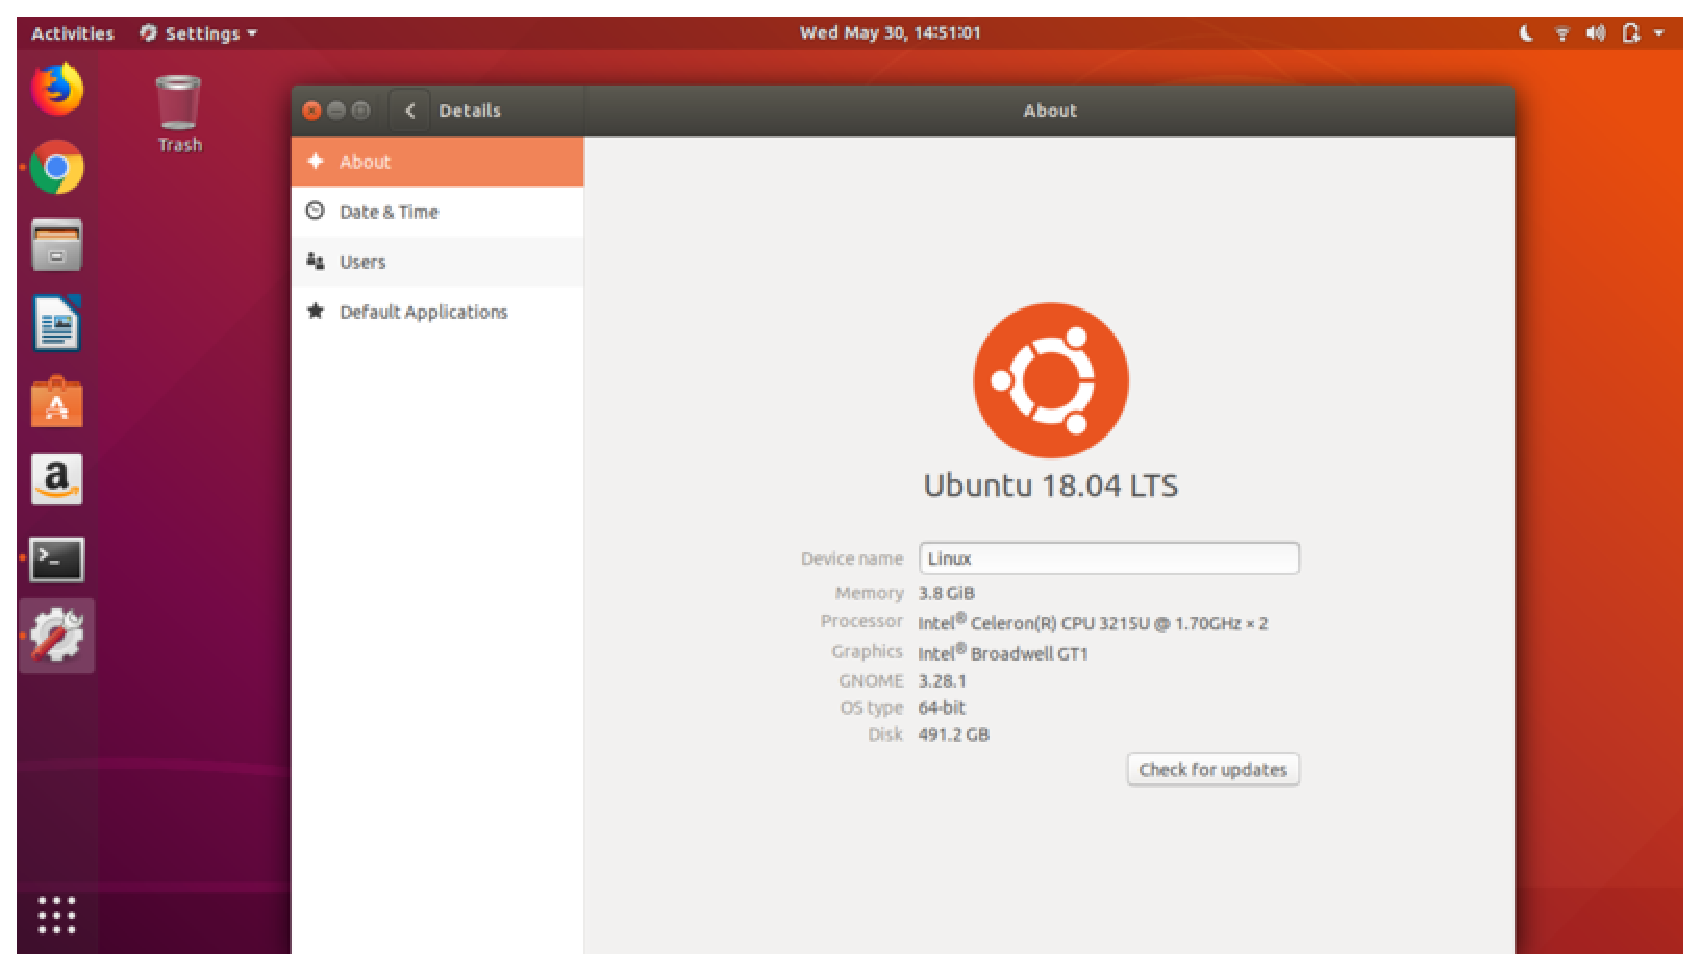
\includegraphics[scale=.5]{Ubuntu-18.04.eps}
%		\caption{Linux Ubuntu version 18.04 desktop.}
%		\label{fig:ubuntu}
%	\end{figure}
%\end{center}

\paragraph{Kali Linux}is a Linux distribution for penetration
testers. It consists of many widely used tools for pentest. This
distribution make it easy to use common tools in a pentest. There are
about 200+ tools in Kali Linux for various stages of a
pentest. Figure~\ref{fig:kali} show a Kali Linux distributions with
tools for penetration testing.

%\begin{center}
%	\begin{figure}[]
%		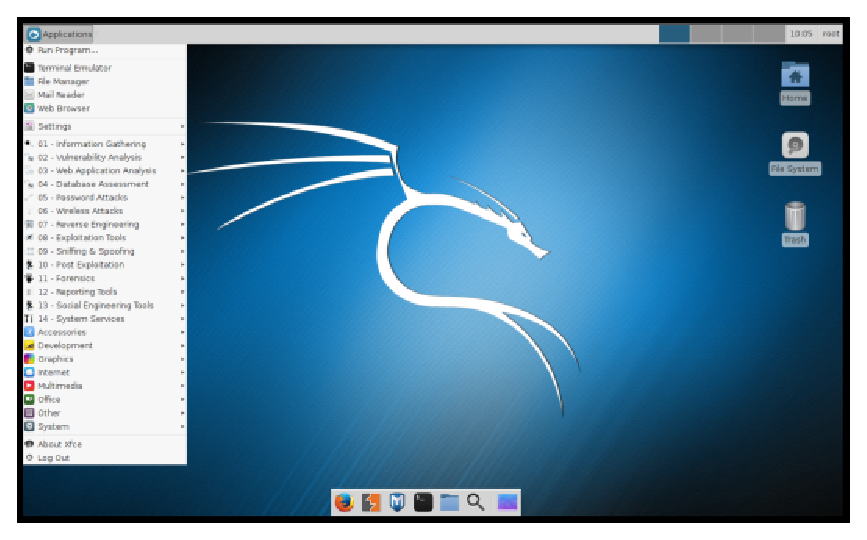
\includegraphics[scale=.5]{kali-linux.eps}
%		\caption{Kali Linux. A Linux distribution for pen testers.}
%		\label{fig:kali}
%	\end{figure}
%\end{center}

\begin{figure*}[!t]
\centering
\subfloat[Kali Linux]{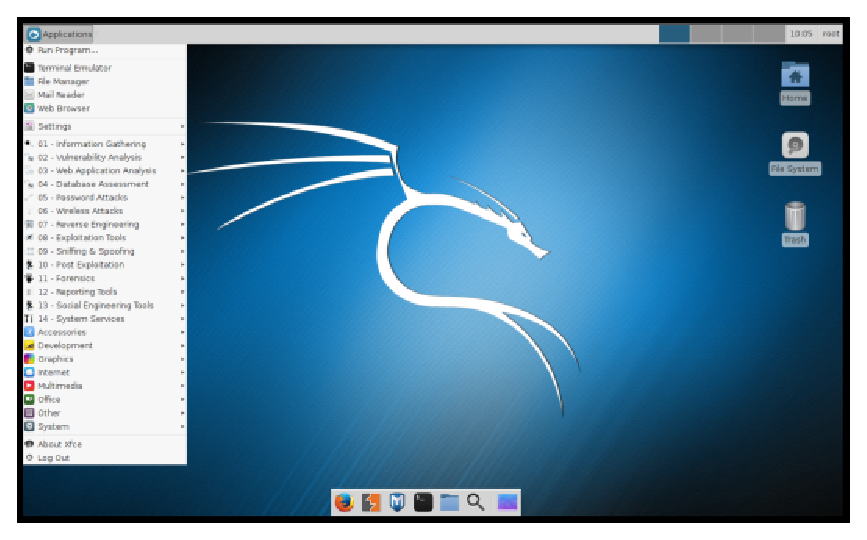
\includegraphics[width=.45\textwidth]{kali-linux.eps}%
\label{fig:kali}}
\hfil
\subfloat[Ubuntu Linux]{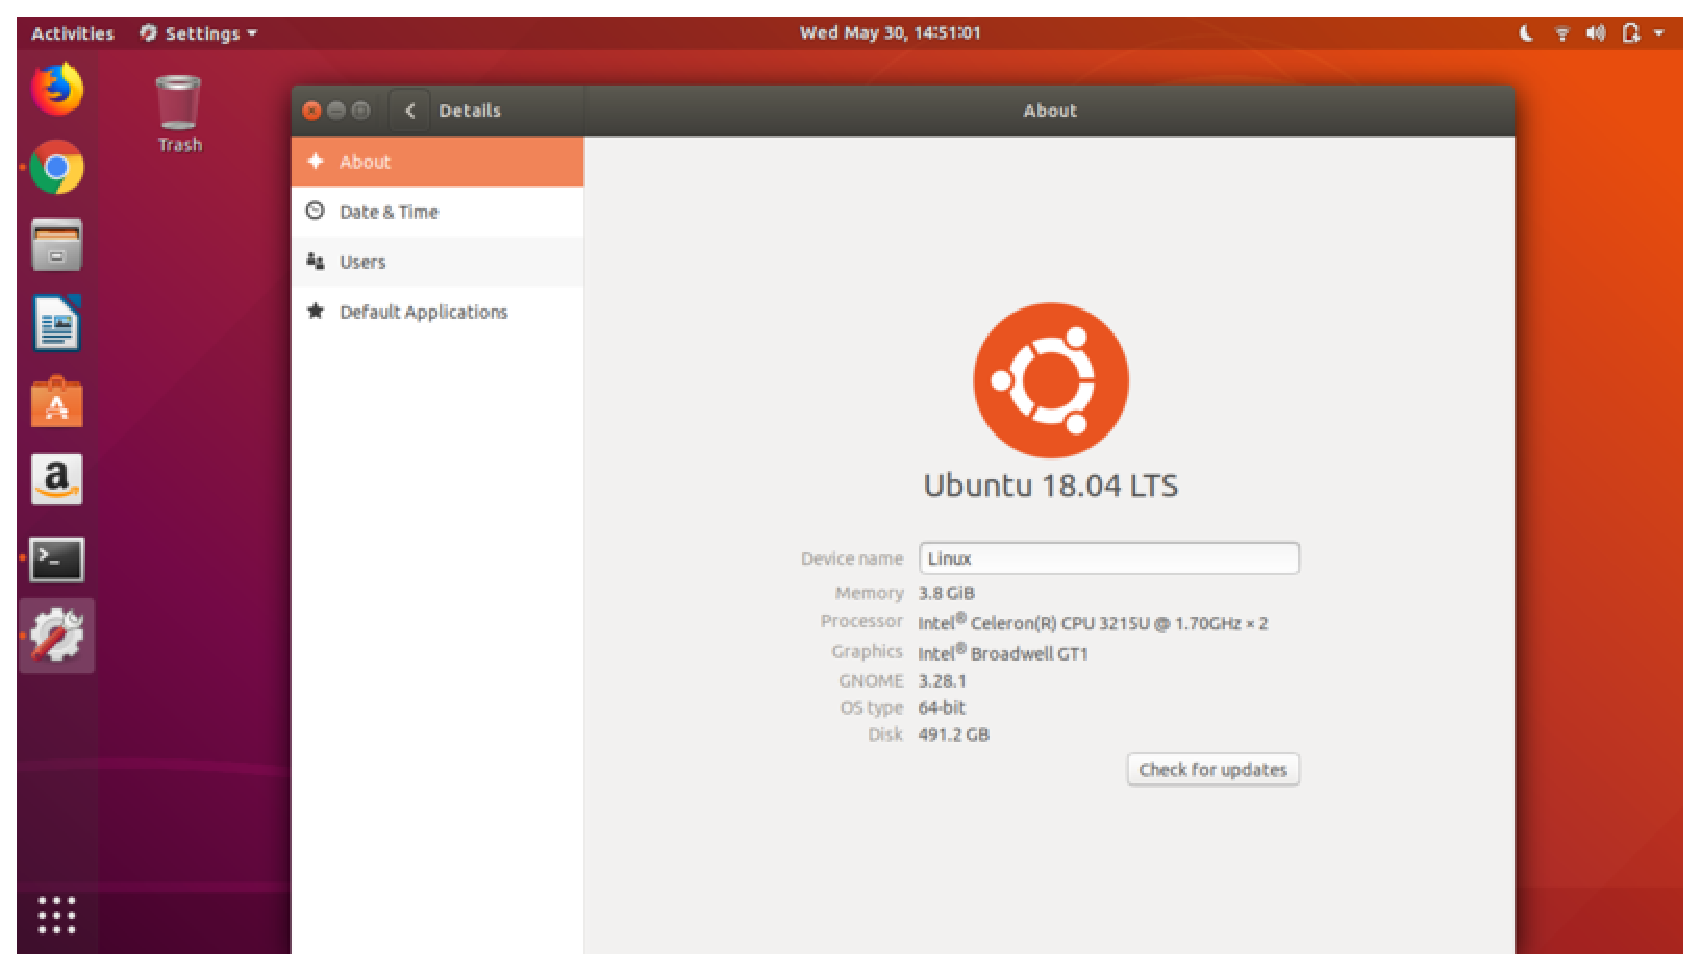
\includegraphics[width=.45\textwidth]{Ubuntu-18.04.eps}%
\label{fig:ubuntu}}
\caption{Example of Linux distributions.}
\label{fig:linux}
\end{figure*}




\section{git}

\paragraph{git}\cite{loeliger2012} is a source code
management tool. \url{github.com} is a git repository, where
software developers share their software source codes in the
Internet. \url{Github.com} host many open source pen test
tools projects such as \url{metasploit} and \url{nmap}. A
pen tester can clone the repository and install the software
on his machine. With this approach, the pen tester can
always use the latest version of the software.

A pen tester need to clone the repository from \url{github.com}. An
example for such action is given below for cloning \url{nmap}
repository. Figure~\ref{fig:github} show a sample repository at
\url{github.com}.


\verb|git clone https://github.com/nmap/nmap.git|

% https://www.online-convert.com/
% take screen shot in png, convert to eps

%\begin{center}
%	\begin{figure}[ht]
%		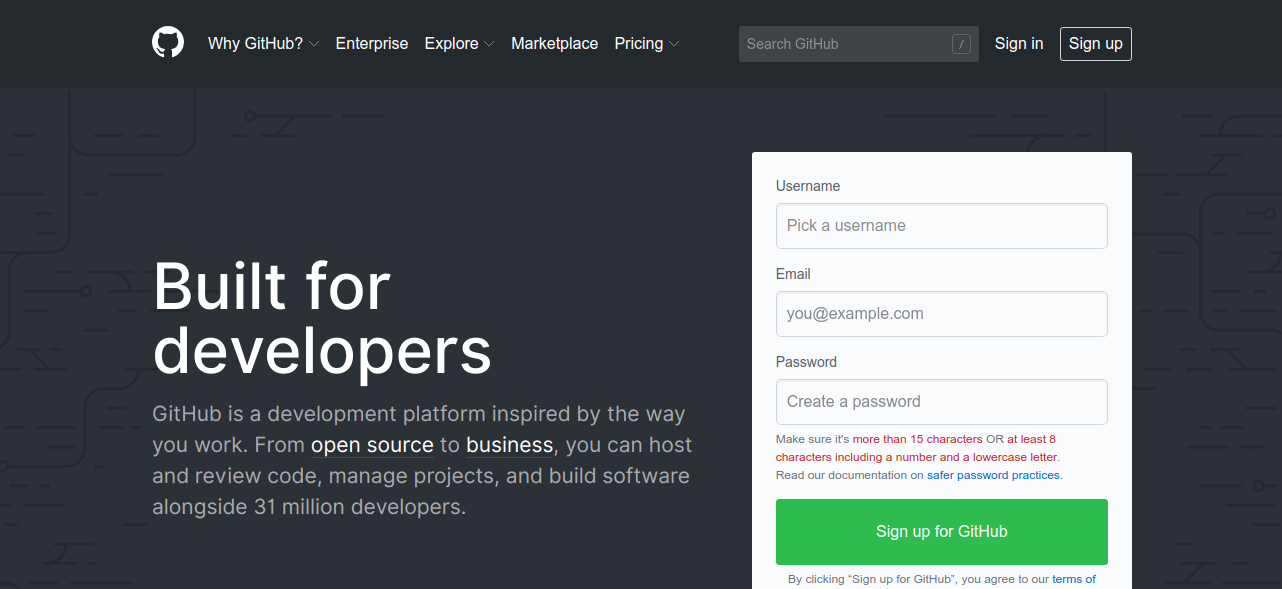
\includegraphics[width=.50\textwidth]{github.eps}
%		\caption{github.com}
%	\end{figure}
%\end{center}

\begin{figure}
\centering
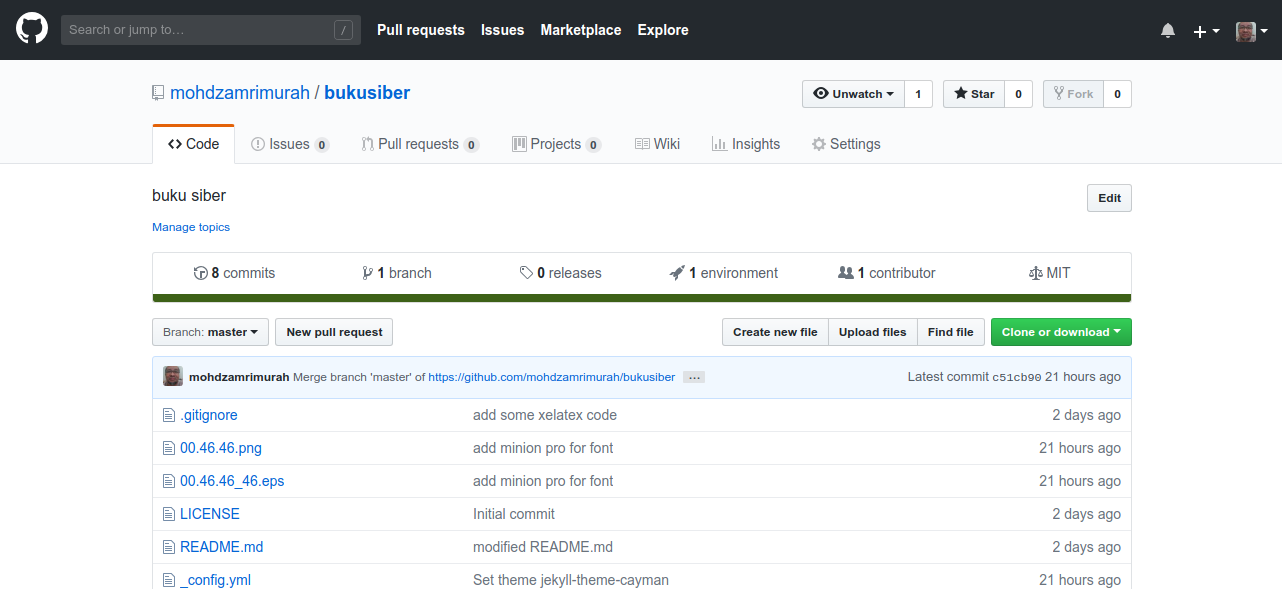
\includegraphics[width=.75\textwidth]{github-ui.eps}
\caption{Source code repository at github.com}
\label{fig:github}
\end{figure}

\index{topics}{git}
\index{authors}{Loeliger, Jon}

\section{Python}

\paragraph{Python}\cite{van2007python,lutz2013learning,lutz2010programming}
is a general-purpose, high-level programming language whose design
philosophy emphasizes code readability. Currently, it is widely used
in data science, deep learning and web development and software
development. It has been used to develop tools for pen tests.  There
are many pen test tools written in Python, hosted at
\url{github.com}. An example is \url{Sublist3r}, a tool for network
scanning and reconnaisance. \index{topics}{Sublist3r}

\index{topics}{Python}
\index{authors}{Lutz, Mark}

Many process in a pen test can be automated using Python. Using
Python, we could developed new tools for pen tests, automated the
process and discovered new vulnerabilties.


%\section{Raspberry Pi}
%
%\paragraph{Raspberry Pi} is a small single-board computer. It can be used 

\section{Cybersecurity News}

\section{Definitions}

\section{Web resources}

There exist tons of materials related to pen-test online. It is best to adopt
a life long attitude toward pen test where one try to always update oneself
with the latest info about pen test. These are some of useful websites;
\begin{enumerate}
\item \url{https://github.com/enaqx/awesome-pentest}
\end{enumerate}


\section{Cybersecurity Accreditation}



\section{Summary}

\begin{center}
	\begin{figure}[ht]
		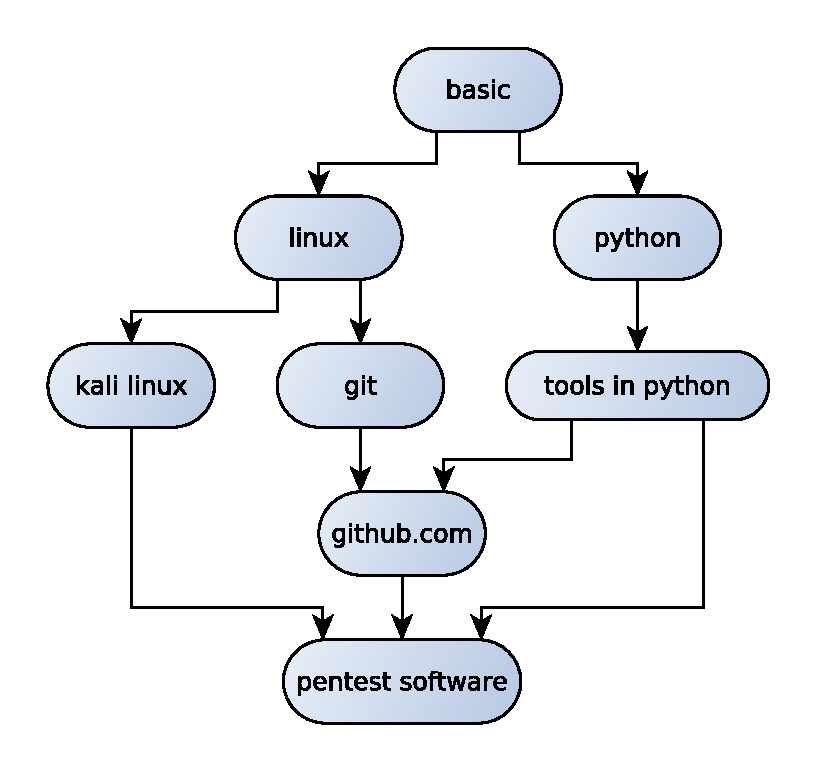
\includegraphics[scale=.75]{tools.eps}
		\caption{Basic tools for pen testers.}
	\end{figure}
\end{center}




\chapternotes



\chapter{Network Basic}

% based on SANS540

\section{Network}
\section{How Internet works}
\section{IP, DNS}
\section{Web servers}


\chapter{Network}

\section{Reconnaissance}
\section{Scanning}
\section{Enumeration}
\section{Vulnerability Assessment}



\chapter{Web Apps}
\section{Web Apps}
\section{Reconnaissance}
\section{Scanning}
\section{Enumeration}
\section{Vulnerability Assessment}

\chapter{Wireless}



\chapter{Mobile}

\chapter{Server and Desktop}

%\nocite{*}
%\bibliographystyle{mit-chicago}
\bibliographystyle{unsrt}
\bibliography{buku}


\printindex{authors}{Author Index}
\printindex{topics}{Topic Index}

\end{document}
